\documentclass[12pt]{report}
\usepackage[utf8]{inputenc}
\usepackage[english]{babel}
\usepackage[letterpaper, portrait, margin=1in]{geometry}
\usepackage{amsmath}
\numberwithin{equation}{section}
\usepackage{amssymb}
\usepackage{graphicx}
\usepackage{parskip}
\usepackage{xcolor}
\usepackage{physics}
\usepackage{empheq}
\usepackage{cancel}
\usepackage{hyperref}
\hypersetup{colorlinks = true, urlcolor = blue, linkcolor = red, citecolor = red}
\usepackage{enumerate}
\usepackage{tikz}
\usepackage{float}
\usepackage{tcolorbox}
\usepackage{booktabs}
\usepackage[bottom]{footmisc}
\usepackage{amsthm}
\usepackage{enumitem}

\newcommand{\unit}[1]{\hat{\boldsymbol{#1}}}
\newcommand{\bd}[1]{\boldsymbol{#1}}
\renewcommand{\b}[1]{\boldsymbol{#1}}
\renewcommand{\vec}[1]{\boldsymbol{#1}}

\definecolor{dmb}{HTML}{003366}

\theoremstyle{definition}
\newtheorem{theorem}{Theorem}[section]
\newtheorem{definition}[theorem]{Definition}
\newtheorem{claim}[theorem]{Claim}
\newtheorem{proposition}[theorem]{Proposition}
\newtheorem{lemma}[theorem]{Lemma}
\newtheorem{corollary}[theorem]{Corollary}
\newtheorem{conjecture}[theorem]{Conjecture}
\newtheorem{example}[theorem]{Example}

\DeclareMathOperator{\spann}{span}
\DeclareMathOperator{\nulll}{null}
\DeclareMathOperator{\range}{range}


\begin{document}
	
	\title{\textbf{Linear Algebra: A Brief Overview\newline\normalsize From \textit{Linear Algebra Done Right} by Sheldon Axler }}
	\author{\textbf{Yi J. Zhu}}
	\date{Month Date, 2021\\\vspace{1em}\small Updated \today}
	\maketitle
	\thispagestyle{empty}
	
	\tableofcontents
	
	\chapter{Vector Spaces}
	
	\section{Fields}
	
	Fields are an important structure that come up in the study of linear algebra. We shall define them below.
	
	\begin{definition}[Field]
		A field is a set of elements $ \mathbb{F} $ with two binary operations, addition $ + $ and multiplication $ \cdot $, that satisfies the field axioms for all $ x,y,z\in \mathbb{F} $, 
		\begin{enumerate}[label=C\arabic*, start=1]   
			\item \textbf{(Closure under addition)} $ x+y \in \mathbb{F} $
			\item \textbf{(Closure under multiplication) } $ x\cdot y \in \mathbb{F} $
		\end{enumerate}
		\begin{enumerate}[label=A\arabic*, start=1]   
			\item \textbf{(Commutativity of addition) }$ x+y = y+x $
			\item \textbf{(Associativity of addition)} $ (x+y)+z = x+(y+z) $
			\item \textbf{(Additive identity) }There exists $ 0\in \mathbb{F} $ such that $ x+0=x  $
			\item \textbf{(Additive inverse) }There exists $ -x \in \mathbb{F} $ such that $ x+(-x)=0 $
			\item \textbf{(Commutativity of multiplication)} $ x\cdot y = y\cdot x $
			\item \textbf{(Associativity of multiplication)} $ (x\cdot y)\cdot z = x\cdot (y\cdot z) $
			\item \textbf{(Multiplicative identity)} There exists $ 1\in \mathbb{F} $ such that $ x\cdot 1=x  $ 
			\item \textbf{(Multiplicative inverse) }There exists $ x^{-1} \in \mathbb{F} $ such that $ x\cdot x^{-1}=1 $
			\item \textbf{(Distributivity of multiplication over addition)} $ x\cdot(y+z)  = x\cdot y + x\cdot z$
			\item \textbf{(Distinct additive and multiplicative identities)} $ 1\neq 0 $
		\end{enumerate}
		\label{def:field axiom}
	\end{definition}
	
	Note that the final field axiom excludes one-element sets from being fields. 
	
	Many of the properties of a field are intuitive to our understanding of introductory mathematics. Here are a few properties of interest.
	
	\begin{theorem}[Unique Identity]
		The additive identity 0 and the multiplicative identity 1 are both unique. 
	\end{theorem}

	\begin{proof}
		Additive identity: suppose 0 and $ 0' $ are additive identities,
		\begin{equation}
				0 = 0 + 0' = 0' + 0 = 0'
		\end{equation}
		Multiplicative identity: similarly, suppose 1 and $ 1' $ are multiplicative identities,
		\begin{equation}
				1 = 1\cdot 1' = 1'\cdot 1 = 1'
		\end{equation}
	\end{proof}

	\begin{theorem}[Unique Inverse]
		For $ x\in \mathbb{F} $, the additive inverse $ -x $ and multiplicative inverse $ x^{-1} $ are unique.
	\end{theorem}
	\begin{proof}
		Additive inverse: suppose $ \alpha $ and $ \beta $ are both additive inverses of $ x\in \mathbb{F} $,
		\begin{equation}
				\alpha = \alpha + 0 = \alpha+(x + \beta) = (\alpha + x) + \beta = \beta
		\end{equation}
	Multiplicative inverse: follows the same process as the proof above.
	\end{proof}

\begin{theorem}
	For any $ x,y, z\in \mathbb{F} $, 
	\begin{enumerate}
		\item $ x\cdot 0  = 0$
		\item $ (-1)\cdot x  = -x$
		\item $ (-x)\cdot y = x\cdot(-y) = -(xy) $
		\item $ (-x)\cdot (-y) = xy $
		\item If $ x +z = y+z$, then $ x = y $
		\item If $ xz = yz $ and $ z\neq 0 $, then $ x=y $
	\end{enumerate}
	Where $ xy $ is shorthand for $ x\cdot y $. 
\end{theorem}

\begin{proof}
	(1) For any $ x\in \mathbb{F} $,
	\begin{equation}
			x\cdot 0 = x\cdot (0+0) = x\cdot 0 + x\cdot 0
	\end{equation}
	Thus,
	\begin{equation}
			x\cdot 0 = 0
	\end{equation}

	(2) For any $ x\in \mathbb{F} $, we want to show that $ x + (-1)\cdot x = 0 $,
	\begin{equation}
			x + (-1)\cdot x = 1\cdot x + (-1)\cdot x = (1+(-1))\cdot x = 0\cdot x = 0 
	\end{equation}
	(3-6) is left as an exercise.
\end{proof}

\section{Lists}

\begin{definition}[List]
	A list of length $ n $ (or $ n$-tuple) is an ordered collection of $ n $ elements,
	\begin{equation}
			(x_1, x_2, \dots, x_n)
	\end{equation}
	Two lists are equal if an only if they have the same length and same elements in the same order. Unlike for a set, repeated elements in a list have meaning. 
\end{definition}

\begin{definition}
	$ \mathbb{F}^n $ is the set of all lists of length n containing elements of $ \mathbb{F} $,
	\begin{equation}
			\mathbb{F}^n = \{(x_1,\dots,x_n) : x_j\in \mathbb{F} \text{ for } j = 1, \dots, n\}
	\end{equation}
\end{definition}
For example, we can think of $ \mathbb{F}^2 $ as a plane in $ \mathbb{F} $.

\begin{definition}[0 in $ \mathbb{F}^n $]
	We denote 0 as the list of length $ n $ with coordinates,
	\begin{equation}
			0 = (0,\dots,0)
	\end{equation}
\end{definition}

\begin{definition}[Addition in $ \mathbb{F}^n $]
	We define coordinate-wise addition in $ \mathbb{F}^n $ as,
	\begin{equation}
			(x_1, \dots, x_n) + (y_1, \dots, y_n) = (x_1+y_1, \dots, x_n+y_n)
	\end{equation}
	\label{def:addition_fn}
\end{definition}

\begin{definition}[Scalar Multiplication in $ \mathbb{F}^n$]
	The product of a scalar $ \lambda\in \mathbb{F} $ and a list in $ \mathbb{F}^n $ is computed by multiplying each coordinate of the vector by $ \lambda $,
	\begin{equation}
			\lambda\cdot(x_1, \dots, x_n) = (\lambda\cdot x_1, \dots, \lambda\cdot x_n)
	\end{equation}
	\label{def:multiplication_fn}
\end{definition}

\section{Vector Space}

\begin{definition}[Vector Space]
	A vector space $ V $ over a field $ F $ is a set with the following operations and satisfying the following closure and vector-space axioms, for all $ x,y,z\in V $ and $ \lambda, \alpha, \beta \in \mathbb{F} $,
	
	\begin{enumerate}[label=O\arabic*, start=1]   
		\item \textbf{(Vector addition operation)} $ +: V\times V \to V $
		\item \textbf{(Scalar multiplication operation) } $ \cdot: F\times V \to V $
	\end{enumerate}
	\begin{enumerate}[label=C\arabic*, start=1]   
		\item \textbf{(Closed under vector addition)} $ x+y \in V$
		\item \textbf{(Closed under scalar multiplication) } $ \lambda\cdot x  \in V$
	\end{enumerate}
	\begin{enumerate}[label=A\arabic*, start=1]   
		\item \textbf{(Commutativity of vector addition)} $ x+y = y+x $
		\item \textbf{(Associativity of vector addition) } $ (x+y)+z=x+(y+z) $
		\item \textbf{(Vector additive identity)} There exists $ 0\in V $ such that $ x+0=x  $ 
		\item \textbf{(Vector additive inverse)} There exists $ -x \in V$ such that $ x+(-x)=0 $
		\item \textbf{(Distributivity of vector addition over scalar multiplication)} \\$(\alpha  + \beta)\cdot x = \alpha x+ \beta x$
		\item \textbf{(Associativity of scalar multiplication)} $ (\alpha\beta)\cdot x = \alpha\cdot(\beta x) $
		\item \textbf{(Scalar multiplicative identity)} For $ 1\in F$,  $ 1\cdot x=x  $ 
		\item \textbf{(Distributivity of scalar multiplication over vector addition)} \\$ \lambda(x+y) = \lambda x + \lambda y $
	\end{enumerate}

	Notice that the field over which a vector space is defined only serves to specify the set of scalars. Also note that the simplest vector spaces is the zero vector space, $ \{0\} $, which contains only the zero vector over an arbitrary field.
		
	\label{def:vector_space}
\end{definition}

\begin{definition}[Vector]
	A vector is an element of a vector space.
\end{definition}

\begin{proposition} 
	$ \mathbb{F}^n $ is a vector space over $ \mathbb{F} $
\end{proposition}
\begin{proof}
	We can show that $ \mathbb{F}^n $ satisfies the conditions for a vector space (definition \ref{def:vector_space}) with definitions of addition and scalar multiplication over $ \mathbb{F}^n $ (\ref{def:addition_fn} and \ref{def:multiplication_fn}) and the field axioms (definition \ref{def:field axiom}). The full exercise is left for the reader.
\end{proof}

Note that while all $ \mathbb{F}^n $ are vector spaces, the converse is not true: a vector space does not have to be $ \mathbb{F}^n $. The zero vector space is a simple counterexample---though we can devise all manners of interesting and exotic vector spaces.\footnote{Another counterexample that comes to mind: the vector space of $ 2\times2 $ real matrices over $ \mathbb{R} $ with element-wise vector addition and scalar multiplication. Somewhat confusingly, here we say that a matrix is a ``vector" because it is an element of the vector space.}

The properties of a vector space follow very closely from the properties of a field. Thus, we shall omit the proofs and state some of the highlights,
\begin{theorem}
	For a vector space $ V $ over $ \mathbb{F} $,
	\begin{enumerate}
		\item $ V $ has a unique additive identity, $ 0 $
		\item Each element in $ V $ has a unique additive inverse.
		\item $ 0\cdot \b{v} = 0 $ for all $ v\in V $
		\item $ \lambda\cdot0 = 0 $ for all $ \lambda\in \mathbb{F} $
		\item $ (-1) \cdot \b{v} = -\b{v}$ for all $ v\in V $
	\end{enumerate}
\end{theorem}

\section{Subspaces}

\begin{definition}[Subspace]
	A subset $ U $ of $ V $ is a subspace of $ V $ if $ U $ is also a vector space using the same addition and scalar multiplication as defined on $ V $.
\end{definition}

\begin{proposition}[Conditions for a subspace]
	A subset $ U $ of $ V $ is a subspace if and only if $ U $ satisfies the conditions,
	\begin{enumerate}
		\item $ U $ contains the additive identity, $ 0 $
		\item $ U $ is closed under addition and scalar multiplication
	\end{enumerate}
\label{prop:subspace}
\end{proposition}

\begin{example}
	The subspaces of $ \mathbb{R}^3 $ are precisely $ \{0\} $, all lines in $ \mathbb{R}^3 $ that pass through the origin, and all planes in $ \mathbb{R}^3 $ that intersect the origin.
\end{example}

\subsection{Sum of Subspaces}

\begin{definition}[Sum of Subsets]
	Suppose $ U_1, \dots, U_n $ are subsets of $ V $. The sum of the subsets is the set of all possible sums of an element from each subset,
	\begin{equation}
			(U_1 + \dots + U_n) = \{ (u_1 + \dots + u_n) : u_j\in U_j \}
	\end{equation}
\end{definition}

\begin{theorem}
	Suppose $ U_1, \dots, U_n $ are subspaces of $ V $. Then their sum $ (U_1 + \dots + U_n )$ is a subspace of $ V $. Furthermore, it is the smallest subspace of $ V $ containing $ U_1, \dots, U_n $.
	
	\begin{proof}
		It is simple to show that $ 0 \in (U_1 + \dots + U_n )$ and that $ (U_1 + \dots + U_n)  $ is closed under addition and scalar multiplication. Thus, $ (U_1 + \dots + U_n ) $ is a subspace of $ V $.
		
		$ U_1, \dots, U_n $ are all contained in $ (U_1 + \dots + U_n)$ because the zero vector exists in each subset.\footnote{In the sum $ (u_1+\dots + u_n) $, we can set all but one of the $ u $'s to be the zero vector.} Conversely, every subspace of $ V $ containing $ U_1 ,\dots, U_n $ must contain all elements of $ (U_1 + \dots + U_n)$. Thus, $ (U_1 + \dots + U_n)$ is the smallest subspace of $ V $ containing $ U_1, \dots , U_n $.
	\end{proof}
\end{theorem}

\begin{definition}[Direct Sum]
	Suppose $ U_1, \dots, U_n $ are subspaces of $ V $. Then the sum $ (U_1 + \dots + U_n)$ is a direct sum if each element can be written in only one way as a sum $ (u_1+\dots+u_n) $ where $ u_j\in U_j $. A sum that satisfies this condition is denoted $ (U_1 \oplus \dots \oplus U_n)$.
\end{definition}

\begin{theorem}[Condition for a Direct Sum]
	Suppose $ U_1, \dots, U_n $ are subspaces of $ V $. Then  $ (U_1 + \dots + U_n )$ is a direct sum if an only if the only way to write,
	\begin{equation}
			u_1 + \dots + u_n = 0 \quad \text{for } u_j\in U_j
	\end{equation}
	is by taking each $ u_j = 0 $.
	\label{thm:directsum}
\end{theorem}
\begin{proof}
	First suppose $ (U_1 + \dots + U_n )$ is a direct sum. Clearly, we can write $ (0 + \dots + 0) = 0 $. And by the definition of a direct sum, this must be the only way to write 0 as a sum $ (u_1 + \dots + u_n) $.
	
	Now suppose the only way to write 0 as a sum $ (u_1 + \dots + u_n) $ is by taking each $ u_j=0 $. Let $ v\in  (U_1 + \dots + U_n )$ and suppose that we can write $ v $ as,
	\begin{equation}
		v = u_1 + \dots + u_n= u_1' + \dots + u_n'
	\end{equation}
	Then,
	\begin{equation}
			0 = (u_1-u_1') + \dots + (u_n-u_n') 
	\end{equation}
	But we know that each $ ( u_j-u_j')= 0 $. Thus, $ u_j = u_j' $ and each $ v\in  (U_1 + \dots + U_n )$ has a unique representation.
\end{proof}

\chapter{Finite-Dimensional Vector Spaces}

A large portion of linear algebra focuses on a subset of all possible vector spaces that are finite-dimensional---which we shall define more formally later in the chapter. 

Notation: note that from now on, it will be implicit that $ V $ is a vector space over a field $ \mathbb{F} $.

\section{Span}

\begin{definition}[Linear Combination]
	A linear combination of vectors $ v_1, \dots, v_n\in V $ is a vector of the form,
	\begin{equation}
			v = a_1v_1 + \dots + a_nv_n \quad \text{where }a_j\in \mathbb{F}
	\end{equation}
\end{definition}

\begin{definition}[Span]
	The set of all possible linear combinations of a list of vectors is it's span,
	\begin{equation}
			\spann (v_1, \dots, v_n) = \{(a_1v_1 + \dots + a_nv_n): a_j\in \mathbb{F} \}
	\end{equation}
	The span of the empty list $ () $ is defined to be $ \{0\} $
\end{definition}

\begin{theorem}
	The span of a list of vectors in $ V $ is a subspace. Furthermore, it is the smallest subspace of $ V $ containing all the vectors in the list.
\end{theorem}
\begin{proof}
	First, we wish to show that $ \spann (v_1, \dots, v_n)  $ is a subspace of $ V $. We know that,
	\begin{equation}
			0 = 0\cdot v_1 + \dots + 0 \cdot v_n \in \spann (v_1, \dots, v_n) 
	\end{equation}
	Furthermore, $ \spann (v_1, \dots, v_n)  $ is closed under addition and scalar multiplication because,
	\begin{equation}
			(a_1v_1 + \dots + a_nv_n) + (b_1v_1 + \dots + b_nv_n) = (a_1 + b_1)v_1 +\dots + (a_n + b_n)v_n
	\end{equation}
	\begin{equation}
			\lambda (a_1v_1 + \dots + a_nv_n) = \lambda a_1v_1 + \dots + \lambda a_nv_n
	\end{equation}
	Thus, $ \spann (v_1, \dots, v_n)  $ is a subspace of $ V $.
	
	It is clear that $ \spann (v_1, \dots, v_n)  $ contains $ v_1, \dots, v_n$. Conversely, because subspaces are closed under addition and scalar multiplication, every subspace containing $ v_1, \dots, v_n$ must also contain $ \spann (v_1, \dots, v_n)  $. Thus, the span is the smallest subspace of $ V $ containing all of the vectors  $ v_1, \dots, v_n$.
\end{proof}

\begin{definition}[Finite-Dimensional Vector Space]
	A vector space is finite-dimensional if it spanned by a finite list of vectors. A vector space is infinite-dimensional if it is not finite-dimensional.
	\label{def:fd}
\end{definition}


\section{Linear Independence}

\begin{definition}[Linearly Independent]
	A list of vectors $ v_1, \dots, v_n $ is linearly independent if and only if each vector in $ \spann (v_1, \dots, v_n)  $ has a unique representation as a linear combination of $ v_1, \dots, v_n $. The empty list $ () $ is also defined to be linearly independent.
	\label{def:li}
\end{definition}

\begin{theorem}[Condition for Linear Independence]
	A list of vectors $ v_1, \dots, v_n $ is linearly independent if and only if,
	\begin{equation}
		a_1v_1 + \dots + a_nv_n=0 \quad \text{for }a_j\in \mathbb{F}
	\end{equation}
	implies $ a_j =0 $.
\end{theorem}
\begin{proof}
	The proof is similar to the proof of theorem \ref{thm:directsum}.
\end{proof}

\begin{definition}[Linearly Dependent]
	A list of vectors in $ V $ is linearly dependent if it is not linearly independent. In other words, there exists $ a_j\in \mathbb{F} $ that are not all zero, such that,
	\begin{equation}
			 a_1v_1 + \dots + a_nv_n=0
	\end{equation}
\end{definition}

\begin{lemma}[Linear Dependence Lemma]
	Suppose $ v_1, \dots, v_n $ is a linearly dependent list in $ V $. Then there exists $ k\in\{1, 2, \dots, n\} $ such that,
	\begin{enumerate}
		\item $ v_k\in \spann(v_1, \dots, v_n ) $
		\item The span of the list is unchanged if $ v_k $ is removed.
	\end{enumerate}
	\label{lemma:ld}
\end{lemma}
\begin{proof}
	Left for the reader.
\end{proof}

\begin{theorem}
	In a finite-dimensional vector space, the length of every linearly independent list of vectors is less than or equal to the length of every spanning list of vectors.
	\label{thm:li_length}
\end{theorem}
\begin{proof}
	This follows from the linear dependence lemma \ref{lemma:ld}.
\end{proof}

\section{Bases}

\begin{definition}[Basis]
	A basis of $ V $ is a list of vectors in $ V $ that are linearly independent and spans $ V $. 
\end{definition}

\begin{proposition}[Criterion for Basis]
	If $ v_1, \dots, v_n $ is a basis of $ V $, then every vector in $ V $ can be uniquely represented as a linearly combination of  $ v_1, \dots, v_n $.
\end{proposition}
\begin{proof}
	The proof is closely related to the ideas of linear independence (definition \ref{def:li}) and is left for the reader.
\end{proof}

\section{Dimension}

\begin{theorem}
	Any two bases of a finite-dimensional vector space have the same length. This theorem serves as the motivation for our definition of ``dimension."
\end{theorem}
\begin{proof}
	Suppose $ V $ is finite-dimensional and $ B_1 $ and $ B_2 $ are two bases of $ V $. We know $ B_1 $ is linearly independent in $ V $ and $ B_2 $ spans $ V $. Thus, by theorem \ref{thm:li_length}, the length of $ B_2 $. Interchanging $ B_1 $ and $ B_2 $, we also see that the length of $ B_2 $ is less than or equal to the length of $ B_1 $. Thus, the length of $ B_1 $ is equal to the length of $ B_2 $.
\end{proof}

\begin{definition}[Dimension]
	The dimension of a finite-dimensional vector space (definition \ref{def:fd}) is the length of any basis of the vector space.
\end{definition}

\begin{theorem} The following are a few theorems that follow from the definition of a dimension. We shall state them here without proof.
	\begin{enumerate}
		\item If $ V $ is finite-dimensional and $ U $ is a subspace of $ V $, then $ \dim(U)\leq \dim (V)$
		\item If $ V $ is finite-dimensional, then every linearly independent list of vectors in $ V $ with length $ \dim(V) $ is a basis for $ V $
		\item If $ V $ is finite-dimensional, then every spanning list of vectors in $ V $ with length $ \dim(V) $ is a basis for $ V $
		\item If $ U_1 $ and $ U_2 $ are subspaces of a finite-dimensional vector space, then,
		\begin{equation}
				\dim(U_1 + U_2) = \dim(U_1) + \dim(U_2) - \dim(U_1 \cap U_2)
		\end{equation}
	\end{enumerate}
\end{theorem}

\chapter{Linear Maps}

\begin{definition}[Linear Maps]
	A linear map, or linear transformation, from vector space $ V $ to vector space $ W $\footnote{It is implicit that both vector spaces are over $ \mathbb{F} $.} is an operation $ T:V\to W $ with the properties, for any $ v, v_1, v_2\in V $ and $ \lambda\in \mathbb{F} $
	\begin{enumerate}[label=P\arabic*, start=1]   
		\item \textbf{(Additivity)} $ T(v_1 + v_2) = T(v_1) + T(v_2) $
		\item \textbf{(Homogeneity)} $ T(\lambda\cdot v)  = \lambda \cdot T(v)$
	\end{enumerate}
	
	The set of all possible linear maps from $ V $ to $ W $ is denoted $ \mathcal{L}(V,W) $
\end{definition}

\begin{theorem}[Linear Maps take 0 to 0]
	Suppose $ T\in \mathcal{L}(V,W) $ . Then, $T(0) = 0 $.
	\label{thm:0t0}
\end{theorem}
\begin{proof}
	By additivity,
	\begin{equation}
			T(0) = T(0+0) = T(0) + T(0)
	\end{equation}
	Thus,
	\begin{equation}
			T(0) = 0
	\end{equation}
\end{proof}

\begin{definition}[Algebraic Operations on $ \mathcal{L} (V,W)$]
	Suppose $ S,T\in\mathcal{L}(V,W) $ and $\lambda\in\mathbb{F}$. For all $ v\in V $,
	\begin{enumerate}
		\item The sum is defined as $ (S+T)v = Sv + Tv $
		\item The scalar product is defined as $ (\lambda S) v = \lambda\cdot Sv $
	\end{enumerate}
	Notice that these two conditions are sufficient to show that $ \mathcal{L}(V,W) $ is a vector space. Finally,
	\begin{enumerate}[start=3]
		\item The product of linear maps is defined as $ (ST) u = S(Tu) $ for $ T\in\mathcal{L}(U,V) $, $ S\in\mathcal{K}(V,W) $, and $ u\in U $
	\end{enumerate}
\end{definition}

\begin{theorem}[Algebraic Properties of Linear Maps] For $ T, T_1, T_2\in\mathcal{L}(U,V) $ an $ S, S_1, S_2\in\mathcal{L}(V,W) $,
	\begin{enumerate}
		\item \textbf{Associativity}: $ (T_1T_2)T_3 = T_1(T_2T_3)$)
		\item \textbf{Identity}: $ TI = IT = T $ (notice the first $ I $ is the identity map on $ V$ while the second $ I $ is the identity map on $ W $)
		\item \textbf{Distributive}: $ (S_1 + S_2) T = S_1T + S_2T $ and $ S(T_1 + T_2) = ST_1 + ST_2 $
	\end{enumerate}
\end{theorem}

\section{Null Spaces and Ranges}

\begin{definition}
	For $ T\in\mathcal{L}(V,W) $, the null space of $ T $, $ \nulll T $, is the subset of $ V $ consisting of vectors that $ T $ maps to 0,
	\begin{equation}
		\nulll T = \{v\in V : Tv = 0\}
	\end{equation}
\end{definition}

\begin{theorem}
	For $ T\in\mathcal{L}(V,W) $, $ \nulll T $ is a subspace of $ V $.
\end{theorem}

\begin{proof}
	$ T $ is a linear map, so $ T(0)=0 $ (theorem \ref{thm:0t0}). Thus, $ 0\in\nulll T $.
	
	Suppose $ u,v\in\null T $. Then, $ T(u+v) = T(u) + T(v) = 0 + 0 = 0 $. Thus, $ \nulll T$ is closed under addition. 
	
	Suppose $ u\in\nulll T $ and $  \lambda \in \mathbb{F}$. Then, $ T(\lambda u)  = \lambda T(u) = \lambda 0 = 0$. This, $ \nulll T $ is closed under scalar multiplication.
	
	The conditions of a subspace are met (\ref{prop:subspace}).
\end{proof}

\begin{definition} For $ T $, a function from $ V $ to $ W $, the range of $ T $ is,
	\begin{equation}
			\range T = \{Tv : v\in V\}
	\end{equation}
\end{definition}

\begin{theorem} If $ T\in\mathcal{L}(V,W) $, then range $ T $ is a subspace of $ W $.
\end{theorem}
\begin{proof}
	Since $ T $ is a linear map, $ T(0) = 0 $. Thus, $ 0\in\range T $
	
	If $ w_1, w_2\in \range T $, then there must exist $ v_1, v_2\in V $ such that $ Tv_i = w_i $. Thus, =
	\begin{equation}
			T(v_1+v_2) = T(v_1) + T(v_2) = w_1 + w_2
	\end{equation}
	Hence, $ w_1 + w_2 \in \range T $; $ \range T $ is closed under addition.
	
	If $ w\in\range T $ and $ \lambda\in \mathbb{F} $, then there exists $ v\in V $ such that $ T(v) = w $. Thus,
	\begin{equation}
			T(\lambda v) = \lambda T(v) = \lambda w
	\end{equation}
	Thus, $ T $ is closed under scalar multiplication.
\end{proof}

\begin{definition}[Injective]
	A function $ T: V\rightarrow W $ is injective if $ T(u) = T(v) $ implies $ u=v $. In other words, distinct inputs are mapped to distinct outputs.
\end{definition}

\begin{theorem}
	Let $ T\in \mathcal{L}(V, W) $. $ T $ is injective if and only if $ \nulll T = \{0\} $
\end{theorem}

\begin{definition}[Surjective]
	A function $ T $ from $ V $ to $ W $ is surjective if it's range equals $ W $, 
\end{definition}

\begin{figure}[H]
	\centering
	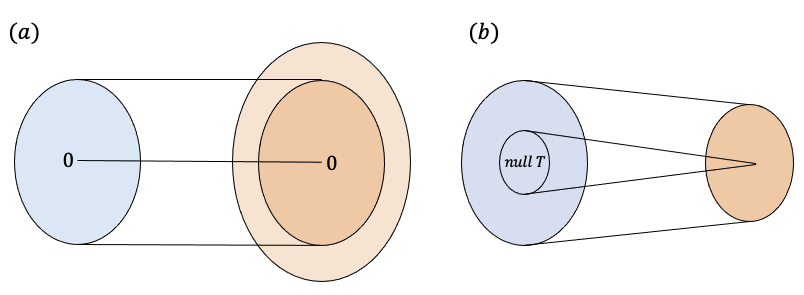
\includegraphics[width=12cm] {img/injsur}
	\caption{Suppose $ T\in\mathcal{L}(V,W) $ is a linear map from $ V $ (blue) to $ W $ (orange) with some $ \range T$ (darker orange). (a) $ T $ is injective. (b) $ T $ is surjective. Notice, a map to a smaller dimensional space can not be injective and a map to a larger dimensional space can not be surjective. We can also show this with the fundamental theorem of linear maps.}
\end{figure}

\section{Fundamental Theorem of Linear Maps}

\begin{theorem}
	Suppose $ V $ is finite-dimensional and $ T\in\mathcal{L}(V, W) $. Then $ \range T $ is finite-dimensional and,
	\begin{equation}
			\dim V = \dim(\nulll T) + \dim(\range T)
	\end{equation}
	\begin{proof}
		Let $ u_1,\dots,u_m $ be a basis of $ \nulll T $. This can be extended to a basis for $ V $,
		\begin{equation}
				u_1, \dots, u_m, v_1, \dots, v_n
		\end{equation}
	
		Thus, $ \dim V = m+n $. To finish, we need to show that $ \dim(\range T)  = n$. We first prove that $ Tv_1, \dots, Tv_n $ is a basis of $ \range T $. For $ a_i, b_j\in \mathbb{F} $,
		\begin{equation}
				v = a_1u_1 + \dots + a_mu_m  + b_1v_1 + \dots + b_nv_n
		\end{equation}
	\begin{align}
			Tv &= T(a_1u_1) + \dots + T(a_mu_m)  + T(b_1v_1) + \dots + T(b_nv_n) \\
			&= b_1T(v_1) + \dots + b_nT(v_n)
	\end{align}

	Thus, $ Tv_1, \dots, Tv_n $ spans $ \range V $. Now, to show that they are linearly independent, suppose $ c_i\in\mathbb{F} $ and, 
	\begin{equation}
			c_1T(v_1) + \dots + c_nT(v_n) = 0
	\end{equation}
	Then,
	\begin{equation}
			T(c_1v_2 + \dots + c_nv_n) = 0
	\end{equation}
	\begin{equation}
			c_1v_2 + \dots + c_nv_n \in \nulll T
	\end{equation}
	Because $ u_1, \dots, u_m $ spans $ \nulll T $,
	\begin{equation}
			c_1v_2 + \dots + c_nv_n  = d_1u_1 + \dots + d_mu_m
	\end{equation}
	But $ u_1, \dots, u_m, v_1, \dots, v_n $ are linearly independent, so $ c_i = d_j = 0 $. Thus, $ Tv_1, \dots, Tv_n $ are linearly independent and span $ \range T $. Hence, $ \dim(\range T) = n $
	\end{proof}

	We have shown that $\dim V = \dim(\nulll T) + \dim(\range T) $
\end{theorem}

\section{Matrices}





\bibliographystyle{ieeetr}
\bibliography{ref.bib}
\nocite{*}
	
\appendix


\end{document}